\documentclass{article}
\title{X16 Edit user manual}
\date{\today}
\usepackage{hyperref}
\usepackage{float}
\usepackage{longtable}
\usepackage{graphicx}
\usepackage{wrapfig}

\begin{document}

\maketitle

\section{Introduction}

    X16 Edit is a simple text editor written in 65C02 assembly especially
    for the Commander X16 retro computer. 
    
    The look and feel of the program is inspired by GNU Nano, but there are,
    naturally, many differences.
    
    One primary design goal is to support editing of large text 
    files. A lot of care has been put into the design of
    the internal memory model to make this possible.

    The Commander X16 was devised by David Murray a.k.a. the 
    8-Bit Guy. For more information on the platform, go to 
    \href{http://www.commanderx16.com}{www.commanderx16.com}.

\section{Getting help}

    X16 Edit is controlled by keyboard shortcuts. The most frequently used 
    shortcuts are always displayed at the bottom of the screen.
    
    There is also a built-in help screen, which is displayed when you press
    Ctrl+G. The help screen lists all keyboard shortcuts with a short description
    of what they do.

    All keyboard shortcuts are also listed in section \ref{commands} of this manual.

\section{Basic usage}

    \subsection{Entering text}
           
        X16 Edit is a modeless editor. As soon as it is started, everything you
        type on the keyboard is inserted into the text buffer.
        
        By default, line breaks are not made automatically. There is no limit
        to the length of a line, other than the available memory. If 
        the current line does not fit on the screen, it is 
        scrolled horizontally. 
        
        There is, however, an optional automatic 
        word wrap mode. Read more about that in section \ref{wordwrap}.
       
    \subsection{Moving the cursor}

        The cursor is primarily moved by the standard arrow keys.

        You may move to start of line with the Home key, and to end of line with Shift+Home.

        The computer does not recognize the standard page up and down keys. Those operations
        are, however, supported by pressing Ctrl+Y (page up) or Ctrl+V (page down).
        
        Finally, it is also possible to move the cursor to a specified line number 
        with the go to line feature (Ctrl+L).

    \subsection{Commands}
    \label{commands}
    
        Commands are selected with keyboard shortcuts. They may be entered in the following three ways:

        \begin{itemize}

            \item Press and hold down the Ctrl key at the same time as you press a command key. This is the
            preferred way of selecting commands.
            
            \item Alternatively you may press and release the Esc key. The progam is now ready to receive
            a command key, and a message stating this is displayed in the status bar. 
            Press a command key, without holding down Ctrl, or Esc to abort. This option is mostly
            made as a backup, in case the Ctrl+key sequence does not work. 
            
            \item Finally, some commands are available via an optional function key.
        \end{itemize}

	\begin{longtable}{c c l}
		\caption{List of keyboard shortcuts} \\
	    \textbf{Ctrl or Esc} & \textbf{F-key} & \textbf{Description} \\
	    \hline \\
            G    & F1    & Display built-in help screen \\
            X    & F2    & Exit from the program \\
            O    & F3    & Write text buffer to file \\
            R    & F4    & Open and read a file into the buffer \\
            N    & ---   & Create new text buffer \\
            Y    & ---   & Page up \\
            V    & ---   & Page down \\
            K    & F5    & Cut current line and save it to clipboard \\
            P    & ---   & Copy current line to clipboard \\
            U    & F6    & Paste (uncut) all content from clipboard \\
            C    & F7    & Display current cursor position (line and column) \\
            W    & F8    & Search and find string in buffer (case sensitive) \\
            S    & ---   & Replace one or all occurrences of a string in buffer (case sensitive) \\
            L    & ---   & Goto line number \\
            A    & ---   & Toggle auto indent on/off \\
            Z    & ---   & Toggle word wrap on/off \\
            E    & ---   & Change charset, cycles through the three supported charsets\\
            D    & ---   & Set file storage device number, default is 8 \\
            T    &  ---  & Cycle through text colors \\
            B    &  ---  & Cycle through background colors \\
            M    &  ---  & Show memory usage (1 block=251 bytes) \\
            space& ---   & Insert non-breaking space 
        \end{longtable}

        \noindent The tab stop width is set by first pressing and releasing Esc and then one of the digits 1--9.

    \subsection{User interface}
	
	The user interface is inspired by GNU Nano, and should be mostly self-explanatory. It consists of the following main parts:
	
	\begin{itemize}
		\item The title bar
		\item The status bar
		\item The shortcut list
		\item The editor area
	\end{itemize}
	
	\noindent The \textit{title bar} is displayed on the first row of the screen. You find the program name and version to the left. 
	The current file name is shown at the center. If the text buffer has never been saved to file, the string "NEW BUFFER" is
	shown instead of a file name. At the right edge, the letters "MOD" are shown if the text buffer has been modified
	since last saved to file.
	
	The \textit{status bar} is the line third from the bottom of the screen. All messages from the program are displayed in
	the status bar. Press Esc to hide a message. If the program needs to prompt you for input, the prompt is also shown in the status bar. 
	Press Enter to confirm input or Esc to abort the operation.
	
	The last two lines at the bottom of the screen contain the \textit{shortcut list}. The most frequently used commands are
	shown here.
	
	The \textit{editor area} covers all lines between the title bar and the status bar. 

    \begin{figure}[H]
        \caption{Main elements of the user interface, (1) title bar, (2) editor area, (3) status bar, and (4) shortcut list.}
        \centering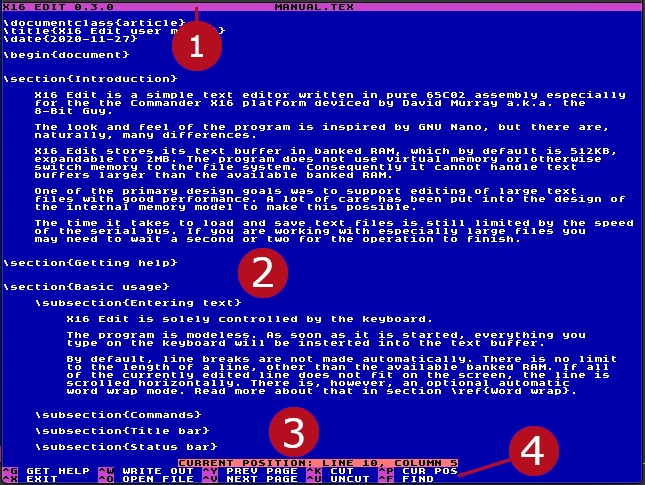
\includegraphics[width=0.67\textwidth]{interface.png}
    \end{figure}
	
	\subsection{Non-breaking space}

        By default, the Commander X16 interprets Shift+space as a non-breaking space. 
        
        To prevent typing errors, the editor will, however, insert a normal space character even if the Shift key is held down.
        Non-breaking spaces are rarely used when you edit raw text files. And it is quite easy to type them by mistake,
        especially if the character immediately before or after the space requires the Shift key.

        If you actually want to insert a non-breaking space you may type Ctrl+space.

    \subsection{Text buffer size}

        X16 Edit stores its text buffer in banked RAM, which by default is 512 kB,
        expandable to 2 MB. 
        
        The program does not use virtual memory or otherwise
        switch memory to the file system. Consequently, it cannot handle text
        buffers larger than the available banked RAM.

        You may get the available free memory by pressing Ctrl+M. The available memory is 
        reported as number of blocks free. One block may hold at most 251 characters.

        If you have used all available memory, the editor will display a memory
        full message in the status bar. Further insertion of characters is ignored.

\section{Features}

    \subsection{Tab stops}

        The default tab stop width is four spaces. You may change the width by pressing and releasing the Esc key followed
        by one of the digits 1--9. The selected digit indicates the tab stop width.
        
        The tab key works by inserting blank spaces until reaching the next tab stop.

    \subsection{Auto indent}
    
        Use the auto indent feature to keep the level of indentation when line breaks are inserted manually or automatically by
        the word wrap feature.

        Auto indent is turned off when the editor starts. To toggle the feature on or off, press Ctrl+A.
    
    \subsection{Automatic word wrap}
    \label{wordwrap}

        By default, automatic word wrap is turned off. If you type a line longer than the width of the screen, the line
        is scrolled horizontally.

        Automatic word wrap is toggled on or off with Ctrl+Z. When turned on, you are prompted for the column where
        to wrap.

        The feature works in a simplified way. When you reach the right margin, the editor breaks the
        line after the previous blank space. If there is no blank space on the line, the line break is inserted
        at the right margin. If you delete characters from a line or if you insert characters at the beginning of a line,
        the line breaks are not recalculated. The feature works well as you type in text, but if you go back and edit that text you
        may have to redo line breaks manually.

    \subsection{Cut, copy and paste}

        X16 Edit supports the traditional cut, copy, and paste features.

        The copy (Ctrl+P) and cut (Ctrl+K) commands copy all of the current line to the clipboard. It is not possible to select 
        a part of a line. The lines you copy or cut are placed in the clipboard in the order they were copied or cut.
        
        The clipboard may hold a maximum of 3 kB of data. If you reach that limit, the program will inform you.

        Pasting or uncutting (Ctrl+U) will insert all content in the clipboard at the position of the cursor. The clipboard
        is cleared after this.

    \subsection{Search and replace}

        X16 Edit also supports search (Ctrl+W) and replace (Ctrl+S).

        Both search and replace are case sensitive. Search starts from the
        cursor position and is only forward looking.

        When searching for a string, the editor moves the cursor to the start
        of the next occurrence. If the string is not found a message is
        displayed in the status bar.

        When replacing a string, you are given the option to only replace the
        next occurrence or all subsequent occurrences.

    \subsection{Supported character sets}

        X16 Edit supports the three character sets of the Commander X16:

        \begin{itemize}
            \item PETSCII upper case/graphics. This is the default mode of both the Commander X16 and the C64.

            \item PETSCII upper/lower case. This is the same mode as is available on the C64.

            \item ISO character set. This mode is new, and there is no corresponding mode supported by 
            Commodore 8 bit computers. Text is encoded according to ISO-8859-15, making it
            easier to transfer files to and from modern computers.
        \end{itemize}

        \noindent On startup, X16 Edit detects the current character set. If the detection is successful, it
        continues using that character set.

        If the current character set for some reason cannot be detected, the program defaults to ISO mode.

        During the operation of the program, it is possible to change the character set. Press Ctrl+E to cycle
        through the options.

    \subsection{Line break encoding}

        The selected character set mode determines how the editor encodes line breaks when writing the
        text buffer to file. 
        
        In both PETSCII modes, it uses a single CR to indicate line breaks. This
        is the closest you get to a standard for Commodore 8 bit computers. This is also the
        setup most likely to work with applications written for Commodore computers.
        
        In ISO mode it uses
        a single LF to mark line breaks. This is the standard used today by Linux and MacOS. Following
        this standard makes it easier to transfer text files to or from modern computers.

        Internally the editor uses a single LF as line break marker. On reading a file it converts
        all occurrences of CR to LF. When writing the text buffer back to file, the line breaks
        are converted to CR if in PETSCII mode.

        In the event you want to save a PETSCII file with LF line breaks or an ISO file with
        CR line breaks, all is not lost. Use the preferred character set mode while
        editing the file. Before saving, switch to ISO mode for LF line breaks or PETSCII mode
        for CR line breaks.

    \subsection{Background and text color}

        Both the background and the text color may be changed while using the editor.

        Press Ctrl+T to cycle through background color options.
        Press Ctrl+B to cycle through text color options.

        \begin{figure}[H]
            \caption{Use your favorite colors!}
            \centering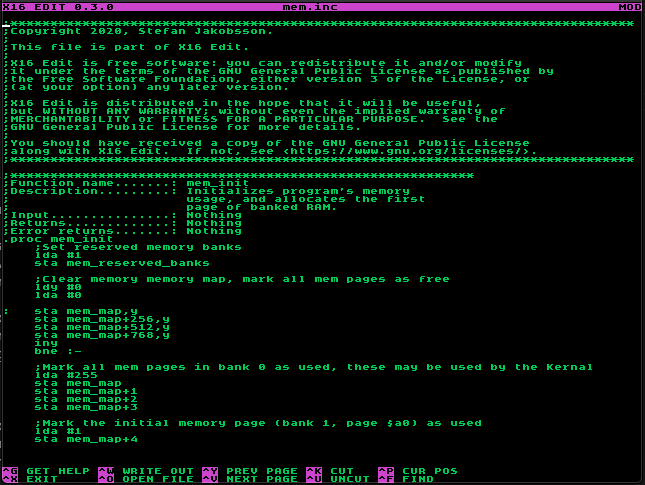
\includegraphics[width=0.5\textwidth]{colors.png}
        \end{figure}
       
\section{File handling}

    X16 Edit supports no other file handling functions than reading (Ctrl+R) and writing files (Ctrl+O).

    In order to simplify the program, there are no functions to show directory listings,
    or to rename, move or delete files. These operations need to be handled at the
    Basic prompt or with other specialized programs.

    By default the program uses device \#8. The device
    number may be changed by pressing Ctrl+D.


\section{License}

	Copyright 2020, Stefan Jakobsson.

	The X16 Edit program, including this manual, is released under the GNU General Public License version 3 or later.
    The program is free software and comes with ABSOLUTELY NO WARRANTY. You may redistribute and/or modify it under the 
    terms of the GNU General Public License as pub­lished by the Free Software Foundation, either version 3 of the License, 
    or, at your option, any later version. For detailed terms see license file distributed with the program. 
    Also available from \href{https://www.gnu.org/licenses}{www.gnu.org/licenses}.

\end{document}